\documentclass[12pt,a4paper]{article}

\usepackage[T2A]{fontenc}
\usepackage[utf8]{inputenc}
\usepackage[english,russian]{babel}
\usepackage{geometry}
\usepackage{graphicx}
\usepackage{booktabs}
\usepackage{amsmath}
\usepackage{hyperref}
\usepackage{float}
\geometry{margin=2.2cm}
\hypersetup{colorlinks=true,linkcolor=blue,urlcolor=blue}
\graphicspath{{results/}}
\renewcommand{\abstractname}{Аннотация}

\title{Моделирование орбитального движения UMKA 1 по модели SGP4}
\author{Практическое задание 3}
\date{22 ноября 2026 г.}

\begin{document}
    \maketitle

    \begin{abstract}
        В работе смоделировано движение спутника UMKA 1 (RS40S), NORAD 57172, по двухстрочным
        элементам орбиты TLE. С помощью библиотеки SGP4 рассчитаны векторы положения и скорости на
        интервале семи суток с шагом 60 секунд. Из векторов получены осциллирующие кеплеровы
        элементы, построена трёхмерная траектория и графики изменения расстояния, скорости и
        элементов орбиты.
    \end{abstract}

    \section{Исходные данные}

    TLE получен из каталога CelesTrak запросом по каталожному номеру 57172. Запись спутника UMKA 1
    (RS40S) на эпоху 22 ноября 2026 года 02:56:23.758 UTC:

    \begin{verbatim}
UMKA 1 (RS40S)
1 57172U 23091G   26326.12249720  .00004205  00000+0  18509-3 0  9999
2 57172  97.4861  24.1939 0010665 290.4673  69.5417 15.22363357188024
    \end{verbatim}

    Основные элементы TLE: $e=0.0010665$, $i=97.4861^\circ$, $\Omega=24.1939^\circ$,
    $\omega=290.4673^\circ$, средняя аномалия $M=69.5417^\circ$, среднее движение $n=15.22363357$
    оборота/сутки. Параметр $B^*=0.00018509$.

    Элементы TLE являются средними элементами, подготовленными для распространения моделью SGP4.

    \section{Методика расчёта}

    Скрипт загружает TLE и создаёт объект \texttt{Satrec}. Для каждого времени $t$ библиотека
    возвращает положение $\mathbf r=(x,y,z)$ в километрах и скорость $\mathbf v=(v_x,v_y,v_z)$ в
    км/с в системе TEME. Интервал равен семи суткам, или 604800 секундам. Включены начало и конец
    интервала, поэтому при шаге 60 секунд вычислено
    \[
    N=\frac{604800}{60}+1=10081
    \]
    состояние. По среднему движению TLE за неделю спутник совершает около $15.22363357\cdot7=106.565$ витка.

    Осциллирующие элементы вычисляются из мгновенных векторов в рамках задачи двух тел. Удельная
    энергия и удельный кинетический момент равны
    \[
    \varepsilon=\frac{v^2}{2}-\frac{\mu}{r},\qquad
    \mathbf h=\mathbf r\times\mathbf v.
    \]
    Затем находятся большая полуось $a=-\mu/(2\varepsilon)$, эксцентриситет
    \[
    e=\left|\frac{\mathbf v\times\mathbf h}{\mu}-\frac{\mathbf r}{r}\right|,
    \]
    наклонение $i=\arccos(h_z/|\mathbf h|)$, долгота восходящего узла $\Omega$ и аргумент перицентра
    $\omega$. Для углов используется функция \texttt{atan2}, учитывающая квадрант. Принято
    $\mu=398600.8\;\mathrm{км^3/с^2}$ и радиус Земли WGS-72 6378.135 км.

    Для модели выбраны константы WGS-72. SGP4 учитывает возмущения земного гравитационного поля,
    включая ведущую зональную составляющую $J_2$, а также эмпирическое влияние атмосферного
    сопротивления через $B^*$. Это распространение модели, заданной TLE, а не отдельное
    численное интегрирование плотности атмосферы и сил.

    \section{Результаты}

    \subsection{Сравнение элементов}

    Большая полуось из среднего движения TLE получена по двухтельной формуле Кеплера
    $a=(\mu/n^2)^{1/3}$, где $n$ переведено из оборотов в сутки в радианы в секунду. В таблице
    \ref{tab:compare} сопоставлены параметры TLE и осциллирующие элементы в начале моделирования.
    Разность углов приведена по кратчайшей дуге.

    \begin{table}[H]
        \centering
        \caption{Средние элементы TLE и начальные осциллирующие элементы}
        \label{tab:compare}
        \begin{tabular}{lrrr}
            \toprule
            Параметр & TLE & Осциллирующий & Разность \\
            \midrule
            $a$, км & 6876.853 & 6883.270 & +6.417 \\
            $e$ & 0.0010665 & 0.0008586 & $-0.0002079$ \\
            $i$, град & 97.4861 & 97.4809 & $-0.0052$ \\
            $\Omega$, град & 24.1939 & 24.1939 & $\approx 0$ \\
            $\omega$, град & 290.4673 & 5.3187 & +74.8514 \\
            \bottomrule
        \end{tabular}
    \end{table}

    Средние элементы TLE не обязаны совпадать с мгновенными осциллирующими элементами:
    преобразование состояния включает короткопериодические составляющие возмущений, которые
    усреднены в TLE. Большая разность аргумента перицентра связана также с малым эксцентриситетом.
    При почти круговой орбите направление перицентра определено слабо, поэтому $\omega$ чувствителен
    к небольшим изменениям вектора эксцентриситета.

    \subsection{Траектория, расстояние и скорость}

    За семь суток моделирование охватывает около 107 витков. Расстояние от центра Земли меняется от
    6875.778 до 6882.516 км, модуль скорости — от 7.60560 до 7.61628 км/с.

    \begin{figure}[H]
        \centering
        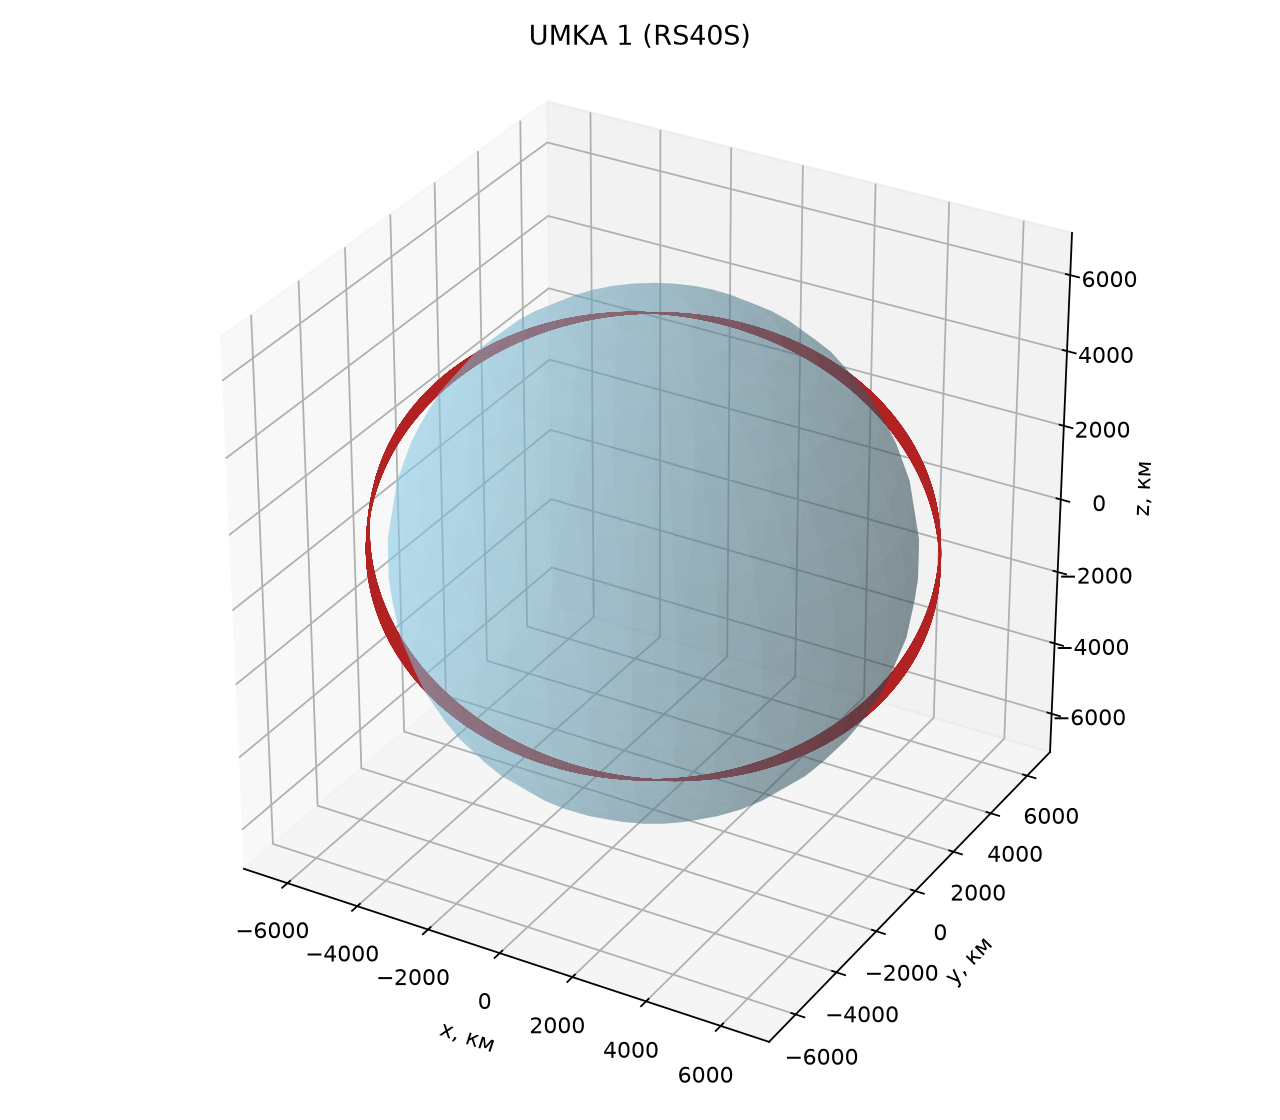
\includegraphics[width=0.76\textwidth]{trajectory_3d.png}
        \caption{Трёхмерная траектория UMKA 1 в системе TEME за 7 суток.}
        \label{fig:orbit}
    \end{figure}

    \begin{figure}[H]
        \centering
        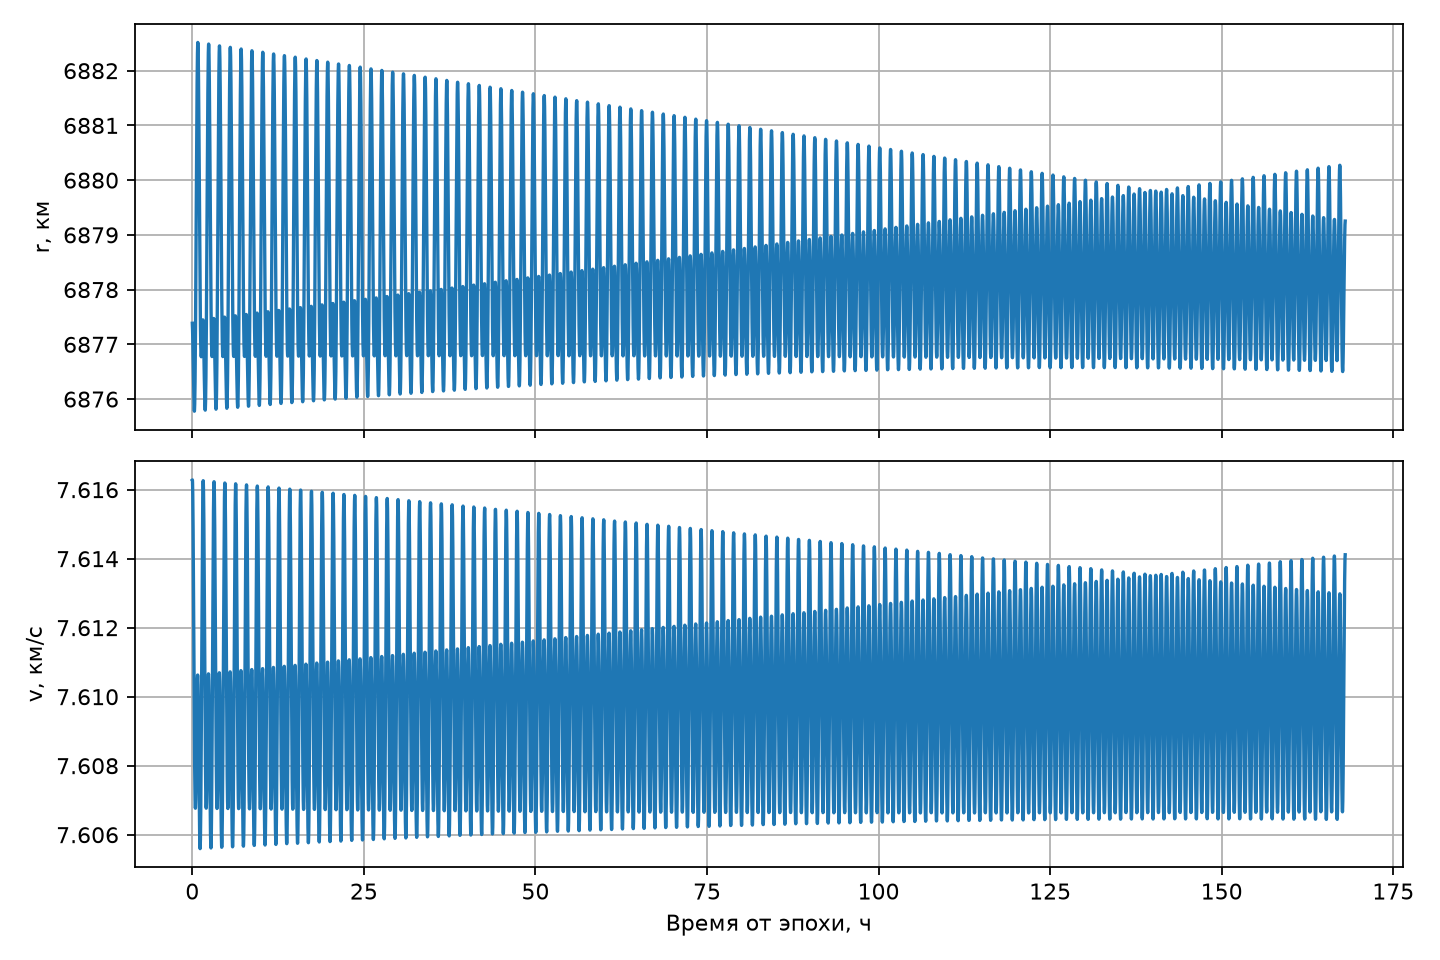
\includegraphics[width=0.92\textwidth]{radius_speed.png}
        \caption{Расстояние от центра Земли и модуль скорости.}
        \label{fig:rv}
    \end{figure}

    \subsection{Осциллирующие элементы во времени}

    Диапазоны элементов и изменение между началом и концом показаны в таблице \ref{tab:change}. Угол
    $\Omega$ развёрнут через границу $360^\circ$. Аргумент $\omega$ оставлен в стандартном диапазоне
    $[-180^\circ,180^\circ]$, так как при малом $e$ его развёртка неустойчива.

    \begin{table}[H]
        \centering
        \caption{Изменение осциллирующих элементов за 7 суток}
        \label{tab:change}
        \begin{tabular}{lrrr}
            \toprule
            Параметр & Минимум & Максимум & Конец минус начало \\
            \midrule
            $a$, км & 6864.208 & 6883.270 & $-0.184$ км \\
            $e$ & 0.000099 & 0.001954 & $-0.000301$ \\
            $i$, град & 97.480926 & 97.491274 & $\approx 0$ \\
            $\Omega$, град & 24.1939 & 31.1647 & $+6.9708^\circ$ \\
            $\omega$, град & $-179.959$ & 179.918 & не показательно \\
            \bottomrule
        \end{tabular}
    \end{table}

    \begin{figure}[H]
        \centering
        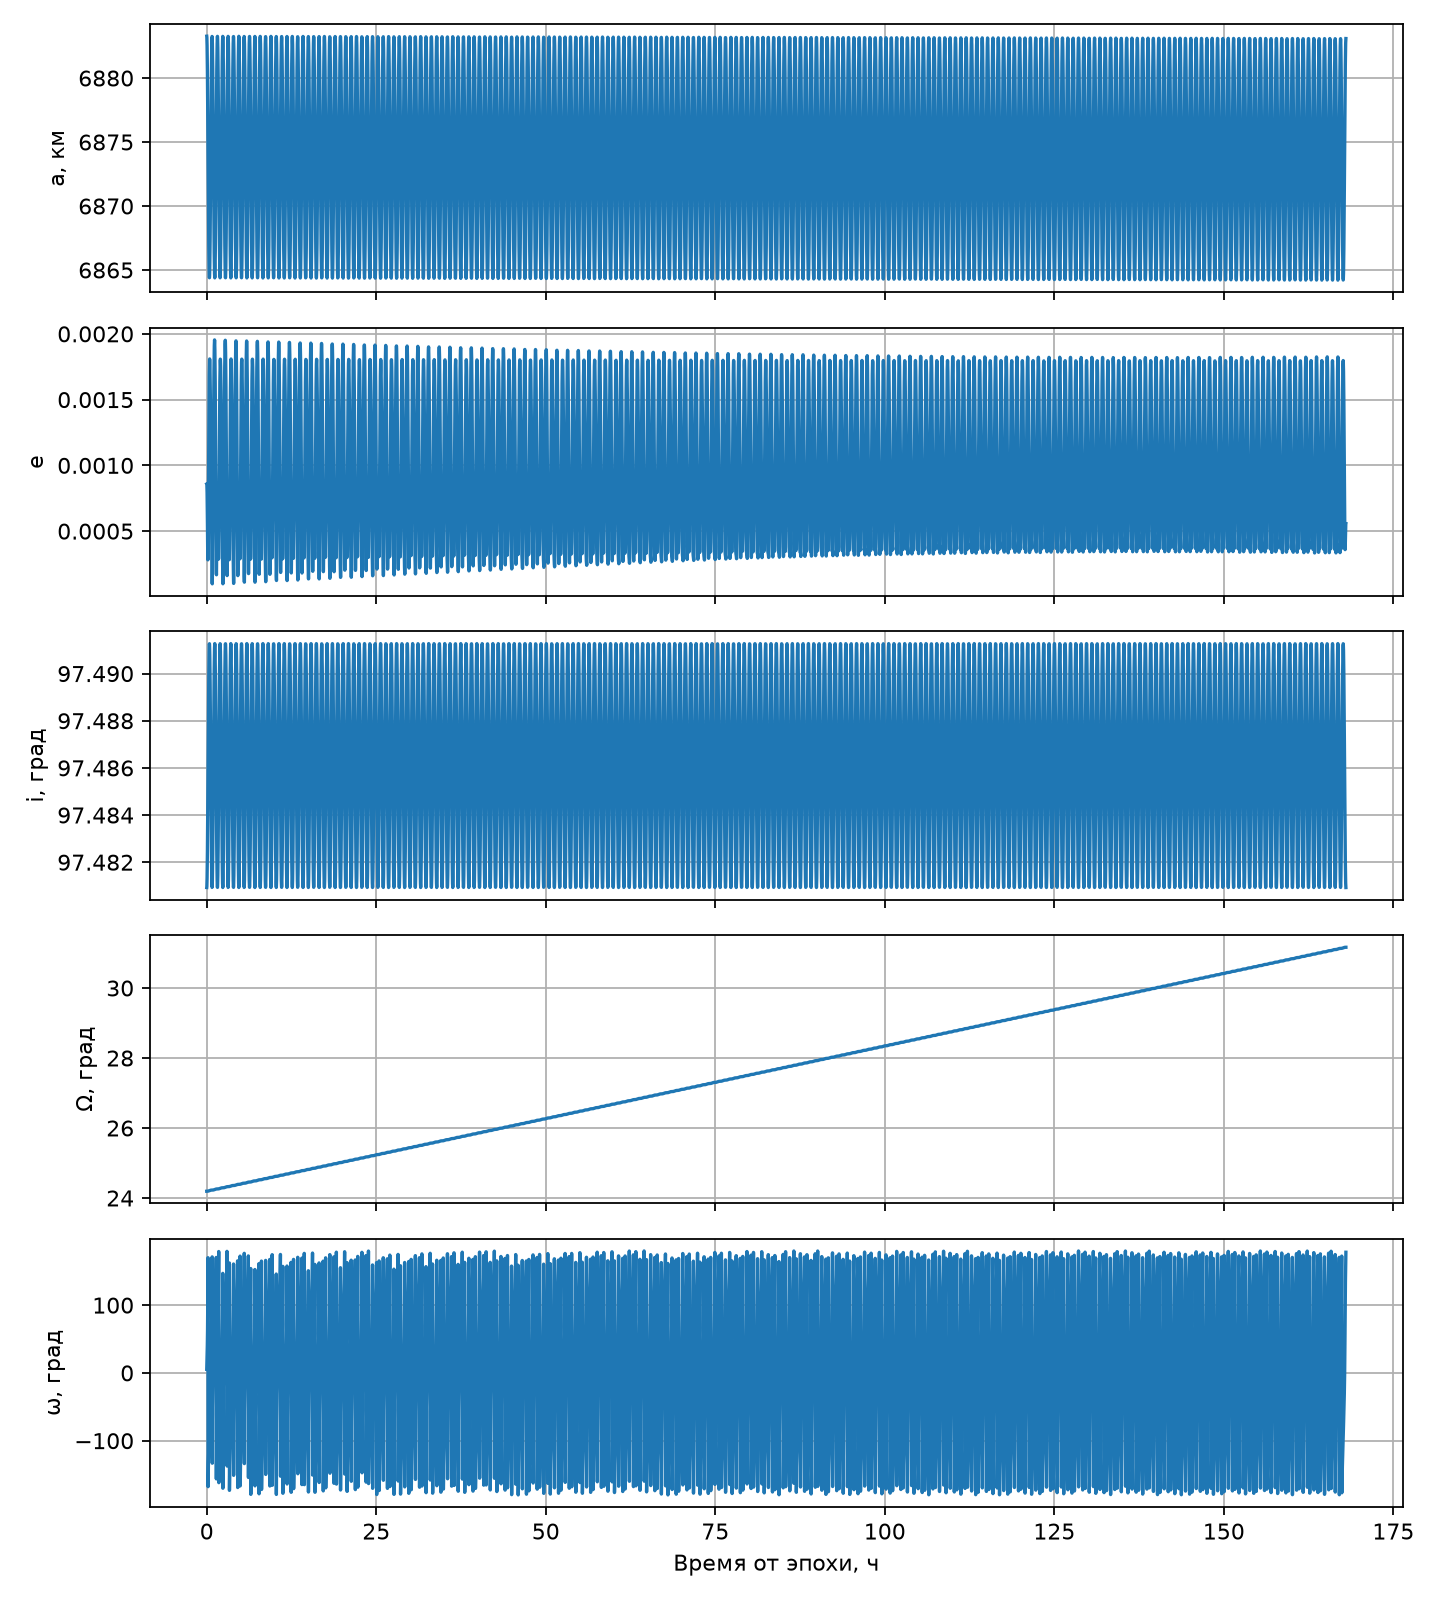
\includegraphics[width=0.92\textwidth]{osculating_elements.png}
        \caption{Осциллирующие элементы, вычисленные из состояния SGP4.}
        \label{fig:elements}
    \end{figure}

    Наклонение практически постоянно. Долгота восходящего узла увеличилась примерно на $6.97^\circ$
    за семь суток (около $1.00^\circ$/сутки); изменение согласуется с влиянием $J_2$ для почти
    полярной ретроградной орбиты. Колебания $a$ и $e$ в основном имеют периодический характер и
    проявляются при преобразовании мгновенного состояния в двухтельные осциллирующие элементы.
    Эксцентриситет мал, поэтому график $\omega$ меняется резко и не даёт надёжной оценки
    долговременного вращения линии апсид. Положительный $B^*$ означает, что SGP4 включает тормозной
    член, но изменение осциллирующих элементов нельзя отождествлять с чистым эффектом сопротивления:
    одновременно действуют гравитационные возмущения и короткопериодические составляющие.

    \section{Выводы}

    \begin{enumerate}
        \item Для UMKA 1 (NORAD 57172) рассчитано 10081 состояние с шагом 60 секунд за семь суток.
        За это время спутник совершает около 107 витков. Его орбита близка к круговой: расстояние
        от центра Земли находится в пределах 6875.778--6882.516 км, а скорость —
        7.60560--7.61628 км/с.

        \item Начальная осциллирующая большая полуось равна 6883.270 км, что на 6.417 км больше
        оценки по среднему движению TLE. Это ожидаемое различие средних элементов TLE и мгновенных
        двухтельных элементов, полученных из векторов SGP4; оно включает короткопериодические
        составляющие возмущений.

        \item Долгота восходящего узла $\Omega$ увеличилась на $6.9708^\circ$ за семь суток.
        Такой сдвиг согласуется с влиянием несферичности Земли, прежде всего члена $J_2$, на
        почти полярную ретроградную орбиту. Большая полуось, эксцентриситет и наклонение при этом
        испытывают периодические колебания.

        \item Эксцентриситет мал, поэтому аргумент перицентра $\omega$ чувствителен к малым
        изменениям вектора эксцентриситета. Его резкие изменения на графике нельзя без
        дополнительных данных трактовать как надёжное вращение линии апсид.

        \item Атмосферное сопротивление представлено в SGP4 эмпирическим параметром $B^*$.
        Рассчитанное изменение элементов включает также гравитационные и периодические эффекты,
        поэтому по нему одному нельзя выделить величину атмосферного торможения.
    \end{enumerate}

    \section*{Воспроизводимость}

    В папке проекта выполните \texttt{python simulate\_orbit.py}. Скрипт использует сохранённый TLE
    из \texttt{data/tle\_57172.txt}, выводит основные параметры в терминал и сохраняет графики в
    \texttt{results/}. Для нового расчёта можно заменить содержимое файла TLE; численные значения
    отчёта после этого также нужно обновить. Использованы Python, NumPy, Matplotlib и библиотека
    \texttt{sgp4}.

\end{document}
